\ifx\mathnotes\undefined
    \providecommand{\notesroot}{../..}
    \providecommand{\calculusroot}{.}

    \title{微积分}
    \author{Donald Cheung\\jianzhang9102@gmail.com}
    \date{\today\footnote{文档编写开始于2017年11月10日}}

    \documentclass[a4paper,10pt]{ctexbook}
\usepackage{xeCJK}
\usepackage{fontspec}
\usepackage{minted}
\usepackage[CJKbookmarks,colorlinks,linkcolor=red]{hyperref}
\usepackage{geometry}
\usepackage{amsmath}
\usepackage[format=hang,font=small,textfont=it]{caption}
\usepackage{float}
\usepackage{subfigure}
\usepackage[nottoc]{tocbibind}
\usepackage{bm}
\usepackage[table, x11names, dvipsnames]{xcolor}
\usepackage{color}
\usepackage{array, booktabs, boldline}
\usepackage{cellspace}
\usepackage{longtable}

\setmainfont{Times New Roman}
\setsansfont{Helvetica}
\setmonofont{Courier New}
\setCJKmainfont[BoldFont={SimHei},ItalicFont={SimHei}]{SimSun}
\setCJKsansfont{SimSun}
\setCJKmonofont{SimSun}

\setcounter{secnumdepth}{4}
\setcounter{tocdepth}{4}

\geometry{left=3.0cm,right=3.0cm,top=2.5cm,bottom=2.5cm}
\bibliographystyle{plain}

%%%%%%%%%%%%%%%%%%%%%%%%%%%%%%%%% minted setting %%%%%%%%%%%%%%%%%%%%%%%%%%%%%%%%%%%
\usemintedstyle{monokai}
\definecolor{bg}{HTML}{282828} % from https://github.com/kevinsawicki/monokai
%\defaultfontfeatures{}
\newfontfamily\noligsmonofamily[NFSSFamily=noligsmonofamily]{Courier}
\setminted{fontfamily=noligsmonofamily}

\renewcommand{\theFancyVerbLine}{%
    \sffamily \textcolor{Dandelion}{\scriptsize \oldstylenums{\arabic{FancyVerbLine}}}}

\newenvironment{jcode}[3]
{%
    \VerbatimEnvironment
    \begin{listing}[h]%
    \caption{#2}%
    \label{#3}%
    \begin{minted}[xleftmargin=18pt,
                   mathescape,
                   linenos,
                   numbersep=5pt,
                   bgcolor=bg,
                   frame=lines,
                   framesep=2mm,
                   fontsize=\footnotesize]{#1}%
}
{%
    \end{minted}
    \vspace{-25pt}%
    \end{listing}%
}
\renewcommand{\listingscaption}{代码}%from minted
\renewcommand{\listoflistingscaption}{代码列表}% from minted


\newenvironment{myquote}{\begin{quote}\kaishu\zihao{-5}}{\end{quote}}
\newcommand\degree{^\circ}
\newtheorem{thm}{定理}


\begin{document}
\maketitle
\tableofcontents
\listoflistings

\else
    \providecommand{\calculusroot}{\mathroot/calculus}
\fi

\chapter{微积分}
\href{http://dataunion.org/20714.html}{寻找最优参数解:最速下降法,牛顿下降法,阻尼牛顿法,拟牛顿法DFP/BFGS}

\section{梯度下降法}

这一节用来介绍常用的数学优化算法--梯度下降法,以及相关变形。

\href{https://arxiv.org/abs/1609.04747}{An overview of gradient descent optimization algorithms}

\href{http://ruder.io/optimizing-gradient-descent}{An overview of gradient descent optimization algorithms}

\href{https://cs.stanford.edu/~ppasupat/a9online/uploads/proximal_notes.pdf}{Proximal and First-Order Methods for Convex Optimization}


大规模机器学习模型训练相关的材料:
\begin{enumerate}
    \item Facebok: \href{https://arxiv.org/abs/1706.02677}{Accurate, Large Minibatch SGD: Training ImageNet in 1 Hour}
    \item \href{https://www.zhihu.com/question/60874090}{如何评价Facebook Training ImageNet in 1 Hour这篇论文?}
    \item \href{https://arxiv.org/abs/1506.08272}{Asynchronous Parallel Stochastic Gradient for Nonconvex Optimization}
\end{enumerate}


\begin{minted}{python}
w = 0
for i in range(0, n):
    w = w - 0.1 * f'(w)
\end{minted}

\begin{table}[H]
    \begin{tabular}{|l|l|l|l|l|}
        \hline
                                & \textbf{batch} & \textbf{mini-batch} & \textbf{Stochastic} & \textbf{Online} \\
        \hline
        \textbf{训练集}         & 固定       & 固定               & 固定               & 实时更新 \\
        \hline
        \textbf{单次迭代样本数} & 整个训练集 & 训练集的子集       & 单个样本           & 根据具体算法定 \\
        \hline
        \textbf{算法复杂度}     & 高         & 一般               & 低                 & 低 \\
        \hline
        \textbf{时效性}         & 低         & 一般(delta 模型) & 一般(delta 模型) & 高 \\
        \hline
        \textbf{收敛性}         & 稳定       & 较稳定             & 不稳定             & 不稳定 \\
        \hline
    \end{tabular}
\end{table}
        

\subsection{基本原理}

\subsection{相关变形}
我们的目的是希望能够在所有可能的数据集上拿到最好的结果,但实际上我们无法获得所有的数据集。
因此在实际的应用中,我们取得是一个是数据集潜在空间的一个抽样,例如训练集。

梯度下降法有3中变形形式,它们之间的区别为我们在计算目标函数的梯度时使用到多少数据,即抽取的样本不同。
根据数据量的不同,我们在参数更新的精度和更新过程中所需要的时间两个方面做出权衡。


\subsubsection{Batch gradient descent}
Vanilla梯度下降法,又称为批梯度下降法(batch gradient descent),
在整个训练数据集上计算损失函数关于参数 $\theta$ 的梯度:
\[
    \theta = \theta - \eta \cdot \nabla_{\theta}{J(\theta)}
\]
其中,
\[
    J(\theta)=\frac{1}{2m}{\sum_{i=1}^{m}{(h_{\theta}(x^{(i)}) - y^{(i)})^2}}
\]

\[
    g_{t} = \frac{\partial f(x_t)}{\partial x_t}
\]

因为在执行每次更新时,我们需要在整个数据集上计算所有的梯度,所以批梯度下降法的速度会很慢。
同时,批梯度下降法无法处理超出内存容量限制的数据集。
批梯度下降法同样也不能在线更新模型,即在运行的过程中,不能增加新的样本。

批梯度下降法的训练算法如下所示:
\begin{align*}
    & repeate \{ \\
    &    \theta = \theta - \alpha \frac{1}{m}{\sum_{i=1}^{m}{(h_{\theta}(x^{(i)}) - y^{(i)})x^{(i)}}} \\
    & \}
\end{align*}
我们利用梯度的方向和学习率更新参数,学习率决定我们将以多大的步长更新参数。
对于凸误差函数,批梯度下降法能够保证收敛到全局最小值,对于非凸函数,则收敛到一个局部最小值。


\subsubsection{Stochastic gradient descent}
随机梯度下降法(stochastic gradient descent, SGD)根据每一条训练样本$ x^{(i)}$ 和标签 $y^{(i)}$ 更新参数:
\[
    \theta = \theta - \eta \cdot \nabla_{\theta}{J(\theta;x^{(i)};y^{(i)})}
\]

对于大数据集,因为批梯度下降法在每一个参数更新之前,会对相似的样本计算梯度,所以在计算过程中会有冗余。
而SGD在每一次更新中只执行一次,从而消除了冗余。因而,通常SGD的运行速度更快,同时,可以用于在线学习。
SGD以高方差频繁地更新,导致目标函数出现如图 \ref{fig:sgd_fluctuation} 所示的剧烈波动。

\begin{figure}[H]
    \centering
    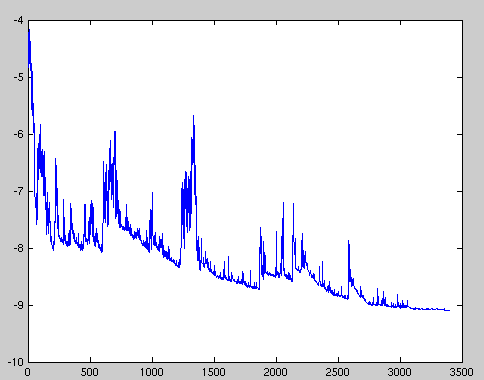
\includegraphics[height=7cm]{\calculusroot/images/sgd_fluctuation.png}
    \caption{SGD波动}
    \label{fig:sgd_fluctuation}
\end{figure}

与批梯度下降法的收敛会使得损失函数陷入局部最小相比,
由于SGD的波动性,一方面,波动性使得SGD可以跳到新的和潜在更好的局部最优;
另一方面,这使得最终收敛到特定最小值的过程变得复杂,因为SGD会一直持续波动。
然而,已经证明当我们缓慢减小学习率,SGD与批梯度下降法具有相同的收敛行为,
对于非凸优化和凸优化,可以分别收敛到局部最小值和全局最小值。
与批梯度下降的代码相比,SGD的代码片段仅仅是在对训练样本的遍历和利用每一条样本计算梯度的过程中增加一层循环。
注意在每一次循环中,最好先随机打乱训练样本。


\subsubsection{Mini-batch gradient descent}
小批量梯度下降法最终结合了上述两种方法的优点,在每次更新时使用$n$个小批量训练样本:
\[
    \theta = \theta - \eta \cdot \nabla_{\theta}{J(\theta;x^{(i:i+n)};y^{(i:i+n)})}
\]

假设训练集有$m$个样本,每个mini-batch(训练集的一个子集)有$b$个样本,
那么,整个训练集可以分成$\frac{m}{b}$个mini-batch。

这种方法,
a) 减少参数更新的方差,这样可以得到更加稳定的收敛结果;
b) 可以利用最新的深度学习库中高度优化的矩阵优化方法,高效地求解每个小批量数据的梯度。

通常,小批量数据的大小在50到256之间,也可以根据不同的应用有所变化。
当训练神经网络模型时,小批量梯度下降法是典型的选择算法,当使用小批量梯度下降法时,也将其称为SGD。


\subsection{相关优化}
虽然Vanilla小批量梯度下降法并不能保证较好的收敛性,但是需要强调的是,这也给我们留下了如下的一些挑战:
\begin{itemize}
    \item 选择一个合适的学习率可能是困难的。
          学习率太小会导致收敛的速度很慢,学习率太大会妨碍收敛,导致损失函数在最小值附近波动甚至偏离最小值。

    \item 学习率调整试图在训练的过程中通过例如退火的方法调整学习率,
          即根据预定义的策略或者当相邻两代之间的下降值小于某个阈值时减小学习率。
          然而,策略和阈值需要预先设定好,因此无法适应数据集的特点。

    \item 此外,对所有的参数更新使用同样的学习率。
          如果数据是稀疏的,同时,特征的频率差异很大时,我们也许不想以同样的学习率更新所有的参数,
          对于出现次数较少的特征,我们对其执行更大的学习率。

    \item 高度非凸误差函数普遍出现在神经网络中,在优化这类函数时,
          另一个关键的挑战是使函数避免陷入无数次优的局部最小值。
          Dauphin等人指出出现这种困难实际上并不是来自局部最小值,
          而是来自鞍点,即那些在一个维度上是递增的,而在另一个维度上是递减的。
          这些鞍点通常被具有相同误差的点包围,因为在任意维度上的梯度都近似为0,所以SGD很难从这些鞍点中逃开。
\end{itemize}

\subsubsection{Momentum}

\[
    \Delta x_{t} = \rho \Delta x_{t-1} - \eta g_{t}
\]

SGD很难通过陡谷,即在一个维度上的表面弯曲程度远大于其他维度的区域,这种情况通常出现在局部最优点附近。
在这种情况下,SGD摇摆地通过陡谷的斜坡,同时,沿着底部到局部最优点的路径上只是缓慢地前进,
这个过程如图 \ref{fig:without_momentum} 所示。

\begin{figure}[H]
    \subfigure[普通SGD]{
        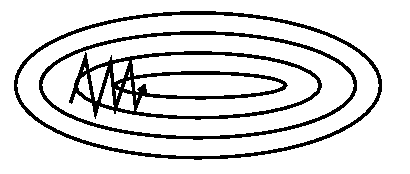
\includegraphics[scale=0.5]{\calculusroot/images/without_momentum.png}
        \label{fig:without_momentum}
    }
    \subfigure[带有冲量的SGD]{
        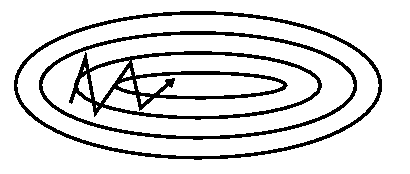
\includegraphics[scale=0.5]{\calculusroot/images/with_momentum.png}
        \label{fig:with_momentum}
    }
    \caption{效果对比图}
\end{figure}

如图 \ref{fig:with_momentum} 所示,动量法是一种帮助SGD在相关方向上加速并抑制摇摆的一种方法。
动量法将历史步长的更新向量的一个分量 $\gamma$ 增加到当前的更新向量中
\begin{align*}
    & v_t = \gamma v_{t-1} + \eta \nabla_{\theta}{J(\theta)} \\
    & \theta = \theta - v_{t}
\end{align*}
动量项 $\gamma$ 通常设置为0.9或者类似的值。

从本质上说,动量法,就像我们从山上推下一个球,球在滚下来的过程中累积动量,变得越来越快
(直到达到终极速度,如果有空气阻力的存在,则 $\gamma < 1$)。
同样的事情也发生在参数的更新过程中:对于在梯度点处具有相同的方向的维度,其动量项增大,
对于在梯度点处改变方向的维度,其动量项减小。
因此,我们可以得到更快的收敛速度,同时可以减少摇摆。


相关实验:\url{https://github.com/hsmyy/zhihuzhuanlan/blob/master/momentum.ipynb}


\subsubsection{Nesterov accelerated gradient}

\url{https://github.com/WarBean/zhihuzhuanlan/blob/master/Momentum_Nesterov.ipynb}

\begin{align*}
    & v_t = \gamma v_{t-1} + \eta \nabla_{\theta}{J(\theta - \gamma v_{t-1})} \\
    & \theta = \theta - v_{t}
\end{align*}




\subsubsection{Adagrad}

\[
    \Delta x_{t} = -\frac{\eta}{\sqrt{\sum_{\tau = 1}^{t}{g_{\tau}^2}}} g_{t}
\]



\subsubsection{RMSprop}
\href{https://arxiv.org/abs/1502.04390}{Equilibrated adaptive learning rates for non-convex optimization}

\begin{align*}
    E[g^2]_{t} = 0.9 E[g^2]_{t-1} + 0.1 g_{t}^2 \\
    \theta_{t+1} = \theta_{t} - \frac{\eta}{\sqrt{E[g^2]_{t} + \epsilon}} g_{t}
\end{align*}



\subsubsection{Adadelta}
在梯度下降法中,学习率是一个需要人为设定的超参数,通常通过人工不断的调整,从而选择效果最好的学习率。
超过这个数值,模型训练的时候无法收敛;小于这个数值,又会导致模型收敛的很慢。
在很多问题中,选择合适的学习率需要靠直觉去选择,没有科学的选择方法。

Adadelta\cite{Zeiler:2012aa} 通过在每个维度上分别引入一个动态的学习率来避免人工选择学习率时遇到的问题。

\[
    E[g^2]_t = \rho E[g^2]_{t-1} + (1 - \rho)g_{t}^2
\]

据说,Adadelta 在深层 RNN 的架构中表现的很好(需要验证)。



\subsubsection{Adam}
\subsubsection{AdaMax}
\subsubsection{Nadam}
\subsubsection{Visualization of algorithms}
\subsubsection{Which optimizer to choose?}

\subsection{Parallelizing and distributing SGD}
\subsubsection{Hogwild!}
\subsubsection{Downpour SGD}
\subsubsection{Delay-tolerant Algorithms for SGD}
\subsubsection{TensorFlow}

\subsubsection{Elastic Averaging SGD}
\subsection{Additional strategies for optimizing SGD}
\subsubsection{Shuffling and Curriculum Learning}
\subsubsection{Batch normalization}

\subsubsection{Early Stopping}
\subsubsection{Gradient noise}


\subsubsection{Online}
随着互联网行业的蓬勃发展,数据变得越来越``廉价''。很多应用有实时的,不间断的训练数据产生。在线学习(Online Learning)算法就是充分利用实时数据的一个训练算法。

Online GD与mini-batch GD/SGD的区别在于,所有训练数据只用一次,然后丢弃。这样做的好处是可以获得模型的变化趋势。比如搜索广告的点击率(CTR)预估模型,网民的点击行为会随着时间改变。用batch算法(每天更新一次)一方面耗时较长(需要对所有历史数据重新训练);另一方面,无法及时反馈用户的点击行为迁移。而Online Leaning的算法可以实时的最终网民的点击行为迁移。

\subsection{深入阅读材料}
\begin{enumerate}
    \item \href{https://arxiv.org/abs/1606.04474}{Learning to learn by gradient descent by gradient descent}



\end{enumerate}






\section{牛顿迭代法}
\subsection{基本原理}
假设 $f(x) = 0$ 为待求解方程,利用传统方法求解,牛顿法求解方程的公式:
\[
f(x_0 + \Delta x) = f(x_0) + f'(x_0)\Delta x
\]
即
\[
    f(x) = f(x_0) + f'(x_0)(x - x_0)
\]

令 $f(x) = 0$,我们能够得到迭代公式:
\[
    x = x_0 - \frac{f(x_0)}{f'(x_0)} \Rightarrow x_{n+1} = x_n - \frac{f(x_n)}{f'(x_n)}
\]
通过逐次迭代,牛顿法将逐步逼近最优值,也就是方程的解。

解决 $f(x) = 0$ 的问题,我们用了一阶泰勒展开:
\[
    f(x) = f(x_0) + f'(x_0)*(x-x_0) + o((x-x_0))
\]
去掉末位高阶展开项,代入 $x = x_0 + \Delta x$,得到:
\[
    f(x) = f(x_0 + \Delta x) = f(x_0) + f'(x_0)\Delta x
\]


那么,要解决 $f'(x) = 0$ 的问题,我们就需要二阶泰勒展开:
\[
    f(x) = f(x_0) + f'(x_0)*(x-x_0) + \frac{f''(x_0)}{2}*(x-x_0)^2 + o((x-x_0)^2)
\]
去掉末位高阶展开项,代入 $x = x_0+\Delta x$,得到:
\[
    f(x) = f(x_0+\Delta x) = f(x_0) + f'(x_0) \Delta x + \frac{f''(x_0) (\Delta x)^2}{2}
\]
求导计算: $f'(x) = f'(x_0+\Delta x) = 0$,得到:
\[
    [f(x_0) + f'(x_0)(x−x_0) + \frac{f''(x_0)(x−x_0)^2}{2}]′ = 0
\]
整理:
\begin{align*}
    & f'(x_0) + f''(x_0)(x−x_0) = 0 \\
    & x = x_0 − \frac{f'(x_0)}{f''(x_0)} \Rightarrow  x_{n+1} = x_n - \frac{f'(x_n)}{f''(x_n)}
\end{align*}

\subsection{拟牛顿条件}

\section{拟牛顿法(Quasi-Newton)}
\subsection{DFP 算法}
\subsection{BFGS算法}
\subsection{L-BFGS 算法}


\section{共轭梯度法(Conjugate Gradient)}
学习资料
\begin{enumerate}
\item《最优化理论与方法》 袁亚湘 孙文瑜
\item http://blog.csdn.net/nocml/article/details/8287466
\item Updating Quasi-Newton Matrices with Limited Storage , Jorge Nocedal
\item Nonlinear Programming, second edition, Dimitri P. Bertsekas
\item《广告数据上的大规模机器学习》  夏粉
\end{enumerate}

\ifx\mathnotes\undefined
    \bibliography{\notesroot/reference/reference.bib}
\end{document}

\fi
